\documentclass[11pt]{report}
\bibliographystyle{ieeetr}
\usepackage[a4paper, total={6in, 8in}]{geometry}
\usepackage{amsmath}
\usepackage[colorlinks=false]{hyperref}
\usepackage{blindtext}
\usepackage{parskip}
\usepackage[nottoc,numbib]{tocbibind}
\usepackage{graphicx} % Required for inserting images
\usepackage[english]{babel}
\usepackage{pdfpages}
\usepackage{xargs}                      % Use more than one optional parameter in a new commands
%\usepackage[pdftex,dvipsnames]{xcolor}  % Coloured text etc.
%
\usepackage[colorinlistoftodos,prependcaption,textsize=tiny]{todonotes}
\newcommandx{\unsure}[2][1=]{\todo[linecolor=red,backgroundcolor=red!25,bordercolor=red,#1]{#2}}
\newcommandx{\change}[2][1=]{\todo[linecolor=blue,backgroundcolor=blue!25,bordercolor=blue,#1]{#2}}
\newcommandx{\info}[2][1=]{\todo[linecolor=OliveGreen,backgroundcolor=OliveGreen!25,bordercolor=OliveGreen,#1]{#2}}
\newcommandx{\improvement}[2][1=]{\todo[linecolor=orange,backgroundcolor=orange!25,bordercolor=orange,#1]{#2}}
\newcommandx{\thiswillnotshow}[2][1=]{\todo[disable,#1]{#2}}

\parskip 2ex
\parindent 0pt

\title{GreenBlocks - SMT PdM}
\author{mbelanger.poly}
\date{August 2023}


\begin{document}

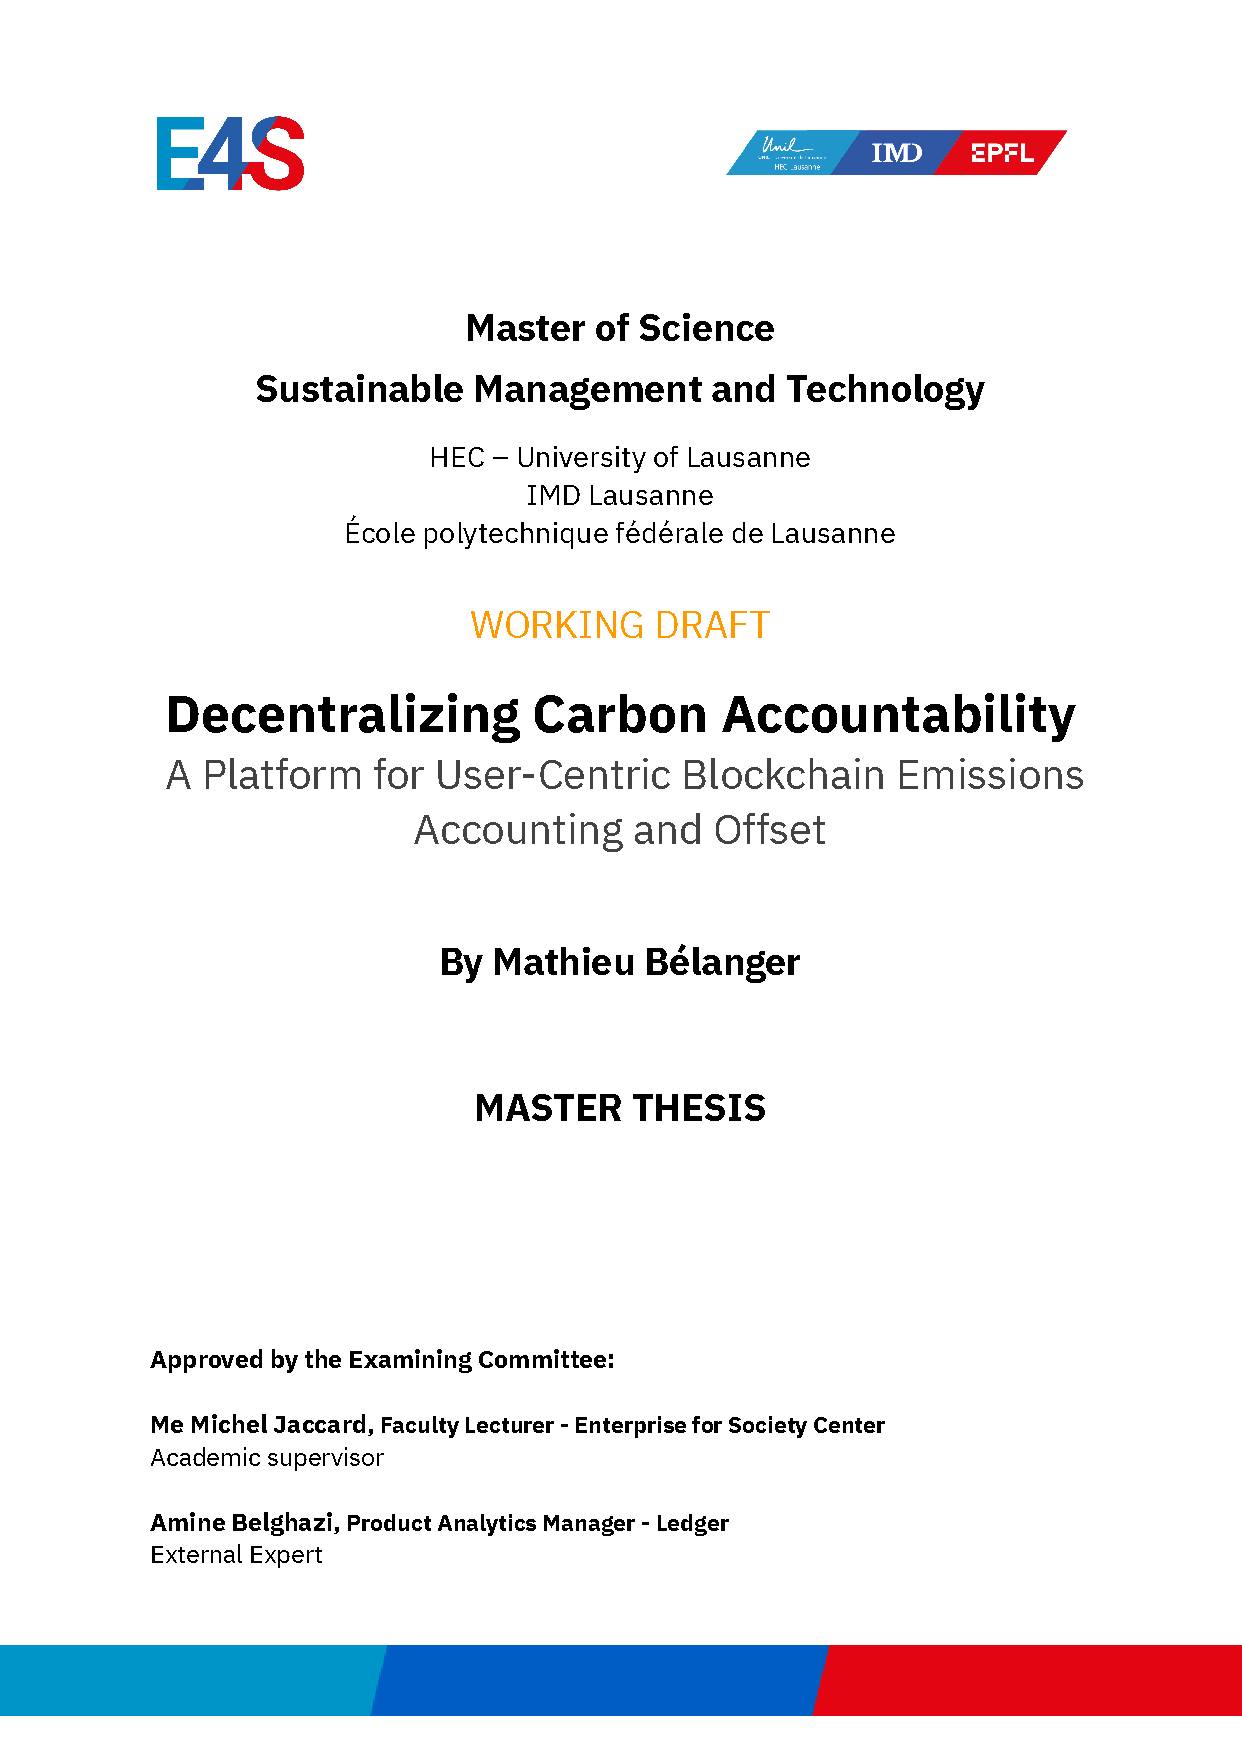
\includepdf[pages={1-2}]{cover.pdf}
\section*{Abstract}
\change{Put abstract in e4s template}
\improvement{Is this too long?}

The advent of blockchain technology has raised concerns about its high energy use and carbon emissions. This is partly due to the current dominance of proof-of-work-driven Bitcoin, which was the first network to gain widespread adoption and media coverage. However, different consensus mechanisms and design choices result in varying environmental footprints across blockchains. While the recent release of the first industry blockchain ESG benchmark enables standardized comparisons between chains at an aggregate level, a granular methodology for user-level emissions accounting is lacking.

This thesis introduces an attribution model designed to map the carbon footprint of blockchain at a user-responsibility level. Novel to this research is the attempt to weigh responsibility factors based on  per-chain estimated importance of different blockchain functions from the perspective of users, capitalizing on the transparency and bounded context of blockchain data. This approach, though unconventional, allows for a more precise and relevant attribution by capturing the relative value users place on different blockchain functionalities. Key factors such as asset balance, transactions signed, and gas spent are used as proxies for user responsibility in overall chain emissions.

\improvement{Unsure. Is the part clear?}

Furthermore, a proof-of-concept tool (GreenBlocks) is built to showcase the attribution model, allowing users
to estimate and offset their emissions through carbon credits. Based on the Ledger Live platform, this
platform interacts seamlessly with leading blockchains and links with on-chain carbon market partners to retire
offsets with maximal transparency.

Greenblocks provides transparent and personalized insights into blockchain emissions for end-users. By
linking usage to quantified environmental impact, it promotes awareness and enables offsets as a means for
users to take responsibility for their use of the technology. Moreover, it demonstrates the potential for
on-chain data to be used as a basis for granular emissions estimation beyond high-level address metrics.
Thus, this thesis proposes a bottom-up, user-focused approach to align blockchain adoption with environmental
sustainability by pioneering user-level footprint attribution.


\change{Add section on further opportunities for the blockchain-sustainability space}

\newpage
\section*{Acknowledgements}
\tableofcontents



\chapter{Introduction}

\section{Background and Motivation}
\improvement{Compartiment in subsections to improve narrative flow}
\subsubsection*{Origins, promise and challenges of blockchain technology}
The advent of blockchain technology since the launch of Bitcoin in 2009 has sparked a revolution in systems of value transfer, transparency, and decentralization \cite{nakamotoBitcoinPeertopeerElectronic2008}. However, the early meteoric rise of cryptocurrencies and underlying blockchain networks has raised critical concerns regarding their environmental sustainability. With the benefit of hindsight, we can view this period as Gartner's Peak of Inflated Expectations. Now, with notorious founders imprisoned, increasing regulatory scrutiny, and the total cryptocurrency market capitalization down 
XX\% from its peak \change{cite}, 
the blockchain ecosystem stands at a crossroads. This is an opportunity to refocus on the core propositions of blockchain technology and ensure its long-term viability.


The dominant network Bitcoin, which utilizes a computationally-intensive proof-of-work consensus mechanism, has attracted particular scrutiny for its high energy consumption. Recent estimates indicate the Bitcoin network alone may consume between 115 and 150 TWh annually, comparable to entire countries like the Netherlands \cite{devriesRevisitingBitcoinCarbon2022,neumuellerCambridgeBitcoinElectricity2021}. This growing apetite for energy competes with the just starting energy transition, putting electrical production and distribution networks under stress. Finally it also results in significant CO2 emissions, hardly compatible with global climate goals like the Paris Climate Accords.

\subsubsection*{Limitations of current approaches}
However, we must recognize the complexity and nuance when evaluating blockchain sustainability. Consensus protocols, design choices, and use cases vary greatly across different networks, leading to wide variability in energy needs and emissions. For instance, proof-of-stake networks like Cardano and Solana promise energy savings by factors of 1000x or more compared to proof-of-work \cite{kohliAnalysisEnergyConsumption2023}. Moreover, Ethereum recently completed its highly anticipated, technically and politically complex transition from proof-of-work to proof-of-stake, demonstrating that such migrations are viable for major networks. \cite{EthereumMergeYour2022} The nascent field of blockchain sustainability analysis must evolve more granular, differentiated perspectives.

Initial responses from the blockchain industry have focused on high-level aggregate comparisons and rankings between networks. For example, recent benchmarks like the Crypto Carbon Ratings Institute methodology provide standardized comparisons of the total lifecycle emissions across chains [5]. However, these overlook the diversity of users and fail to provide accountability at an individual level.

This poses a critical gap, especially as blockchain technology expands into mainstream adoption. We lack a methodology to attribute network-wide emissions to specific users based on their unique activity patterns and values. Such granular carbon accounting can raise awareness of individual impact and empower ethical participation.

\subsubsection*{Opportunities for user-level footprinting}

To address this, the novel approach in this thesis involves an attribution model that weighs factors like asset holdings, transactions, and computations based on their estimated importance to users on each chain. By considering relative user perspectives, we can map emissions more accurately to individual entities like protocols, DAOs, or end-users. This unconventional yet powerful approach unlocks new potentials for transparency, responsibility, and sustainability.

\section{Problem Statement}

As blockchain technology progresses into mainstream integration, the lack of transparency and accountability for emissions at an individual user level poses a critical gap. For example, retail investors drawn to crypto assets may be unaware of the passive environmental impacts associated with their portfolios over time. There is also increasing offering of decentralized applications (web3) with usage beyond those of investing. Granular carbon accounting and attribution to individual wallets can raise awareness and enable offsetting as a means for users to take responsibility of their actions.

Moreover, this gap becomes even more complex for providers of decentralized apps or decentralized autonomous organizations (DAOs) comprising multiple smart contracts and user addresses. Without a methodology for attributing network-wide emissions based on collective usage patterns, a DAO cannot fully assess and mitigate its overall carbon footprint.

Therefore, the overarching problem this thesis addresses is:

"How can we design an attribution model that allocates the carbon emissions of any blockchain network to specific user entities or addresses in a transparent, accurate, and relevant manner based on their unique activity patterns?"

\section{Research Questions and Ojbectives}

To systematically address the problem of transparent and accurate carbon attribution for blockchain users and entities, this thesis pursues four key research questions:

\begin{enumerate}
    \item How can blockchain emission factors be quantified at a granular, user-centric level, beyond aggregate network-wide estimates?
    \item What are appropriate metrics and weighting systems to reflect the responsibilities of diverse blockchain users based on their activities?
    \item How can we validate and demonstrate such an attribution model through a practical implementation?
    \item What are the broader implications of user-centric emissions accounting for accelerating sustainability as blockchain technology matures?
\end{enumerate}

The main objectives of this work are:

\begin{description}

    \item [Develop a User-Level Attribution Model] \hfill \\
    Develop a robust emissions attribution methodology based on usage and responsibility. 
    \item [Greenblock: Pratical Application] \hfill \\
    Implement and validate the model through a functional proof-of-concept application.
    \item [Promote awareness and Responsibility] \hfill \\
    of environmental impact among blockchain users.
    \item [The Future of Sustainability and Blockchain] \change{to complete}
\end{description}

\section{Scope and Limitations}
TO COMPLETE


\section{Structure of the Thesis}
TO COMPLETE

\chapter{Litterature Review}
\section{Economic Externalities}
\section{Evolution of Blockchain Technology}
\section{Environmental Impact of Blockchains}
\subsection{Energy Consumption and Related Emissions}
\subsection{Current Measurement Methodologies and Datasets}
\section{User-Level Emissions Attribution}


\chapter{Methodology: User-Level Emissions Attribution Model}
\section{Overview}

\todo{Find where to include steps of the work. Interviews and data collection}

As blockchain technology advances, a critical question emerges on quantifying and attributing the associated carbon emissions in a transparent manner. While aggregate estimates of blockchain emissions provide a high-level overview, they fail to offer accountability at an individual user level. This poses a major gap in sustainability efforts.

This chapter introduces a methodology to attribute network-wide emissions to specific blockchain addresses based on usage and responsibility factors. By mapping emissions to end-users, protocols, and DAOs, this framework enables entities to understand, report, and take action on their carbon footprints.

A key innovation is the strategy for weighting responsibility factors based on a chain-specific historical measure of blockchains two main features from the user perspective. This captures the nuances of user behavior across diverse blockchains in a relevant, customizable manner. The following sections detail this attribution model and its rationale.

\section{Background}

Blockchains can be categorized into two main types based on their primary function and underlying mechanics:

\begin{description}
    \item[Value Transfer Chains (VTCs)] Chains that focus on transferring assets between addresses (e.g. Bitcoin and derived). VTCs are focused primarily on enabling value transfers through native cryptocurrency tokens. These chains do not typically support complex smart contract functionality like GPCs. The key operational metric for VTCs is the number of transactions, which are constrained by blocksize and block intervals.
    \item[General Purpose Chains (GPCs)] Chains that allow the deployment of smart contracts and decentralized applications (dApps) in addition to value transfer (e.g. Ethereum, Cardano, Solana). On these networks, transactions and computations are quantified using a metric called 'gas'. This concept was introduced by Vitalik Buterin in Ethereum's initial whitepaper \cite{buterinEthereumNextgenerationSmart} as a means to disincentivize computationally intensive smart contracts that could clog the network. Gas puts a cost on network utilization for activities like executing code, storing data, or transferring tokens.
\end{description}

Due to these fundamental differences, GPCs and VTCs require distinct approaches for carbon accounting. On VTCs, the limited blockspace is the bottleneck for transactions. Hence, users conducting more transactions take up a greater share of blockspace and have higher responsibility for the chain's emissions. On GPCs, gas expenditure more accurately reflects utilization and impact on the network's computation and storage load. Users spending more gas have a greater share of responsibility by consuming more of the network's resources and throughput capacity.

Existing studies have estimated blockchain emissions using aggregate network energy use or miner rewards \cite{devriesCryptocurrenciesRoadSustainability2022,devriesRevisitingBitcoinCarbon2022,neumuellerCambridgeBitcoinElectricity2021,mcdonaldEthereumEmissionsBottomup2022}. However, these top-down approaches fail to capture user behavior and responsibility. Our methodology addresses this limitation through a transparent attribution model tailored to GPCs and VTCs using usage factors like gas and transactions. The following sections detail this framework.

\section{Overview of the Attribution Strategy}

\subsubsection*{Objective of the attribution}
A core objective of this methodology is to attribute the carbon emissions of public blockchain networks to individual user addresses. This enables transparency and accountability at a granular level, aligning with sustainability goals. However, accurately and fairly allocating emissions poses significant challenges.

\subsubsection{General Approach}
The strategy involves weighing three responsibility factors - balance, transactions, and gas - based on each chain's historical utility patterns from the user perspective. Specifically, the time series of trading volume is compared to total market capitalization for each chain as proxies for transactional vs holding utility. This aims to capture the relative values users derive from actively transacting on the network versus passively holding assets.

By considering these nuanced dynamics, the methodology differentiates from existing models that apply generic parameters uniformly across diverse blockchain ecosystems. This tailored approach allows for flexible, customizable attribution aligned with actual user behaviors.



\subsubsection*{On Including Passive Holdings as a Responsibility Factor}
A key diffentiator is the inclusion of historical balance as a responsibility factor. Traditionally, emissions accounting ties responsibility to direct actions like executing transactions or computations. \improvement{Add metaphore of traditionnal infrastructure. Roads and km usage vs passive benefit of the road proximity} However, in blockchains, holding assets passively (function of preserving/securing value) also necessitates ongoing mining and transaction fees payed by transacting users, in order to preserve liquidity and value.

\improvement{Put justifications in list form to emphasize each point} 

Specifically, continuous mining activity and block creation are critical to maintain an active market and allow holders to liquidate assets. This activity is incentivized through transaction fees. Higher fees increase miner rewards, resulting in greater security and liquidity that benefit holders.

Therefore, despite no active behavior, holding blockchain assets creates latent demand for emissions-intensive mining. Considering this relationship, the attribution model argues for allocating part of emission responsibility to asset holders, or more generally how intensively a use is using the blockchain function of securing value. 

\section{User-Level Emission Atrribution Model}

Building on the previous overview, this section details the specific components of the emission attribution model.

\subsection{Historical Blockchain Emissions Data}

The emission rate \(E_s(\tau)\) represents the overall amount of tCO2-equivalent emissions generated by the blockchain $s$ at time $\tau$. This is chain-specific, with data aggregated from existing studies \cite{neumuellerCambridgeBitcoinElectricity2021,stollCarbonFootprintBitcoin2019}. 

\todo{Detail combination of papers and dataset access}

\subsection{User attribution parameters}

The responsibility share for an address, owned by a user, is determined based on three factors, in two categories of behavior. Active behavior represents value derived from interacting with the blockchain, while passive behavior represents value derived from holding assets. The three factors are, for an address $addr$ on chain $s$ and at period $\tau$:

\begin{samepage}
\begin{description}
    \item[Active Behavior] \hfill
    \begin{itemize}
        \item[\( \frac{T_{\text{addr}, s}(\tau)}{T_{\text{total},s}(\tau)} \)] Number of transactions as a percentage of total transactions for period $\tau$ (for VTCs)
        \item[\( \frac{G_{\text{addr},s}(\tau)}{G_{\text{total},s}(\tau)} \)] Gas spent as percentage of total gas in blocks for period $\tau$ (for GPCs)
    \end{itemize}
    \item[Passive Behavior] \hfill
    \begin{itemize}
        \item[\( \frac{B_{\text{addr},s}(\tau)}{B_{\text{total},s}(\tau)} \)] Average Balance as a percentage of total token supply on chain $s$ for period $\tau$.
    \end{itemize}
\end{description}
\end{samepage}

\subsection{Weighting factors}
Chain-specific weighting factors $\alpha$, $\beta$, and $\gamma$ account for the different importance of balance, transactions, and gas for each blockchain.

These weights are eastimated by comparing historical time series of trading volume versus market capitalization. Higher relative trading volume indicates users deriving greater utility from transacting versus holding assets.

\improvement{Add formalisation of the weighting factors measurment. Maybe add a figure to illustrate the concept}

\subsection{Attributed Emissions}

Combining the parameters and weights above, the carbon emissions \(A_s(\tau)\) attributed to an address on blockchain $s$ at time $\tau$ is generalized to:

\begin{equation}
    A_{s}(\tau) = E_{s}(\tau) \times 
        [
        \alpha_{s}\frac{B_{\text{addr},s}(\tau)}{B_{\text{total},s}(\tau)} + 
        \beta_{s}  \frac{G_{\text{addr},s}(\tau)}{G_{\text{total},s}(\tau)} + 
        \gamma_{s} \frac{T_{\text{addr},s}(\tau)}{T_{\text{total},s}(\tau)}
        ]
\end{equation}

simplified to:
\improvement{differentiate vars ie Buser Btotal and Bshare to avoid confusion}



\begin{equation}
    A_{s}(\tau) = E_{s}(\tau) \times [\alpha_{s} B(\tau) + \beta_{s} G(\tau) + \gamma_{s} T(\tau)]
\end{equation}

Since we have $\beta_{s} = 0$ for VTCs and $\gamma_{s} = 0$ for GPCs, the attributed emissions on chain $s$ of type $|VTC, GPC|$ are:

\begin{equation}
    A_{VTCs}(\tau) = E_{s}(\tau) \times [\alpha_{s} B(\tau) + \beta_{s} G(\tau)]
\end{equation}

\begin{equation}
    A_{GPCs}(\tau) = E_{s}(\tau) \times [\alpha_{s} B(\tau) + \beta_{s} G(\tau)]
\end{equation}

With $\alpha_{s} + \beta_{s} + \gamma_{s} = 1$ and $\alpha_{s}, \beta_{s}, \gamma_{s} \geq 0$.



\subsubsection*{Cumulative Emissions}

The cumulative emissions $C(t)$ for a user across all his address on chains $S$ up to time $\tau$ is:

\begin{equation}
    C(t) = \sum_{s \in S} \int_{0}^{t} A_s(\tau) d\tau
\end{equation}

This aggregates the attributed emissions across chains over time. The next section concludes this methodology overview.
\improvement{add mention of multiple addresses per chain}

\section{Data Sources and Collection}
\section{Validation and Robustness Analysis}
\subsection{Approach to Validation}
\subsection{Sensitivity Analysis Design}

\chapter{Implementation: GreenBlocks Platform}
\section{Overview}
\begin{figure}[h!]
    \centering
    \centerline{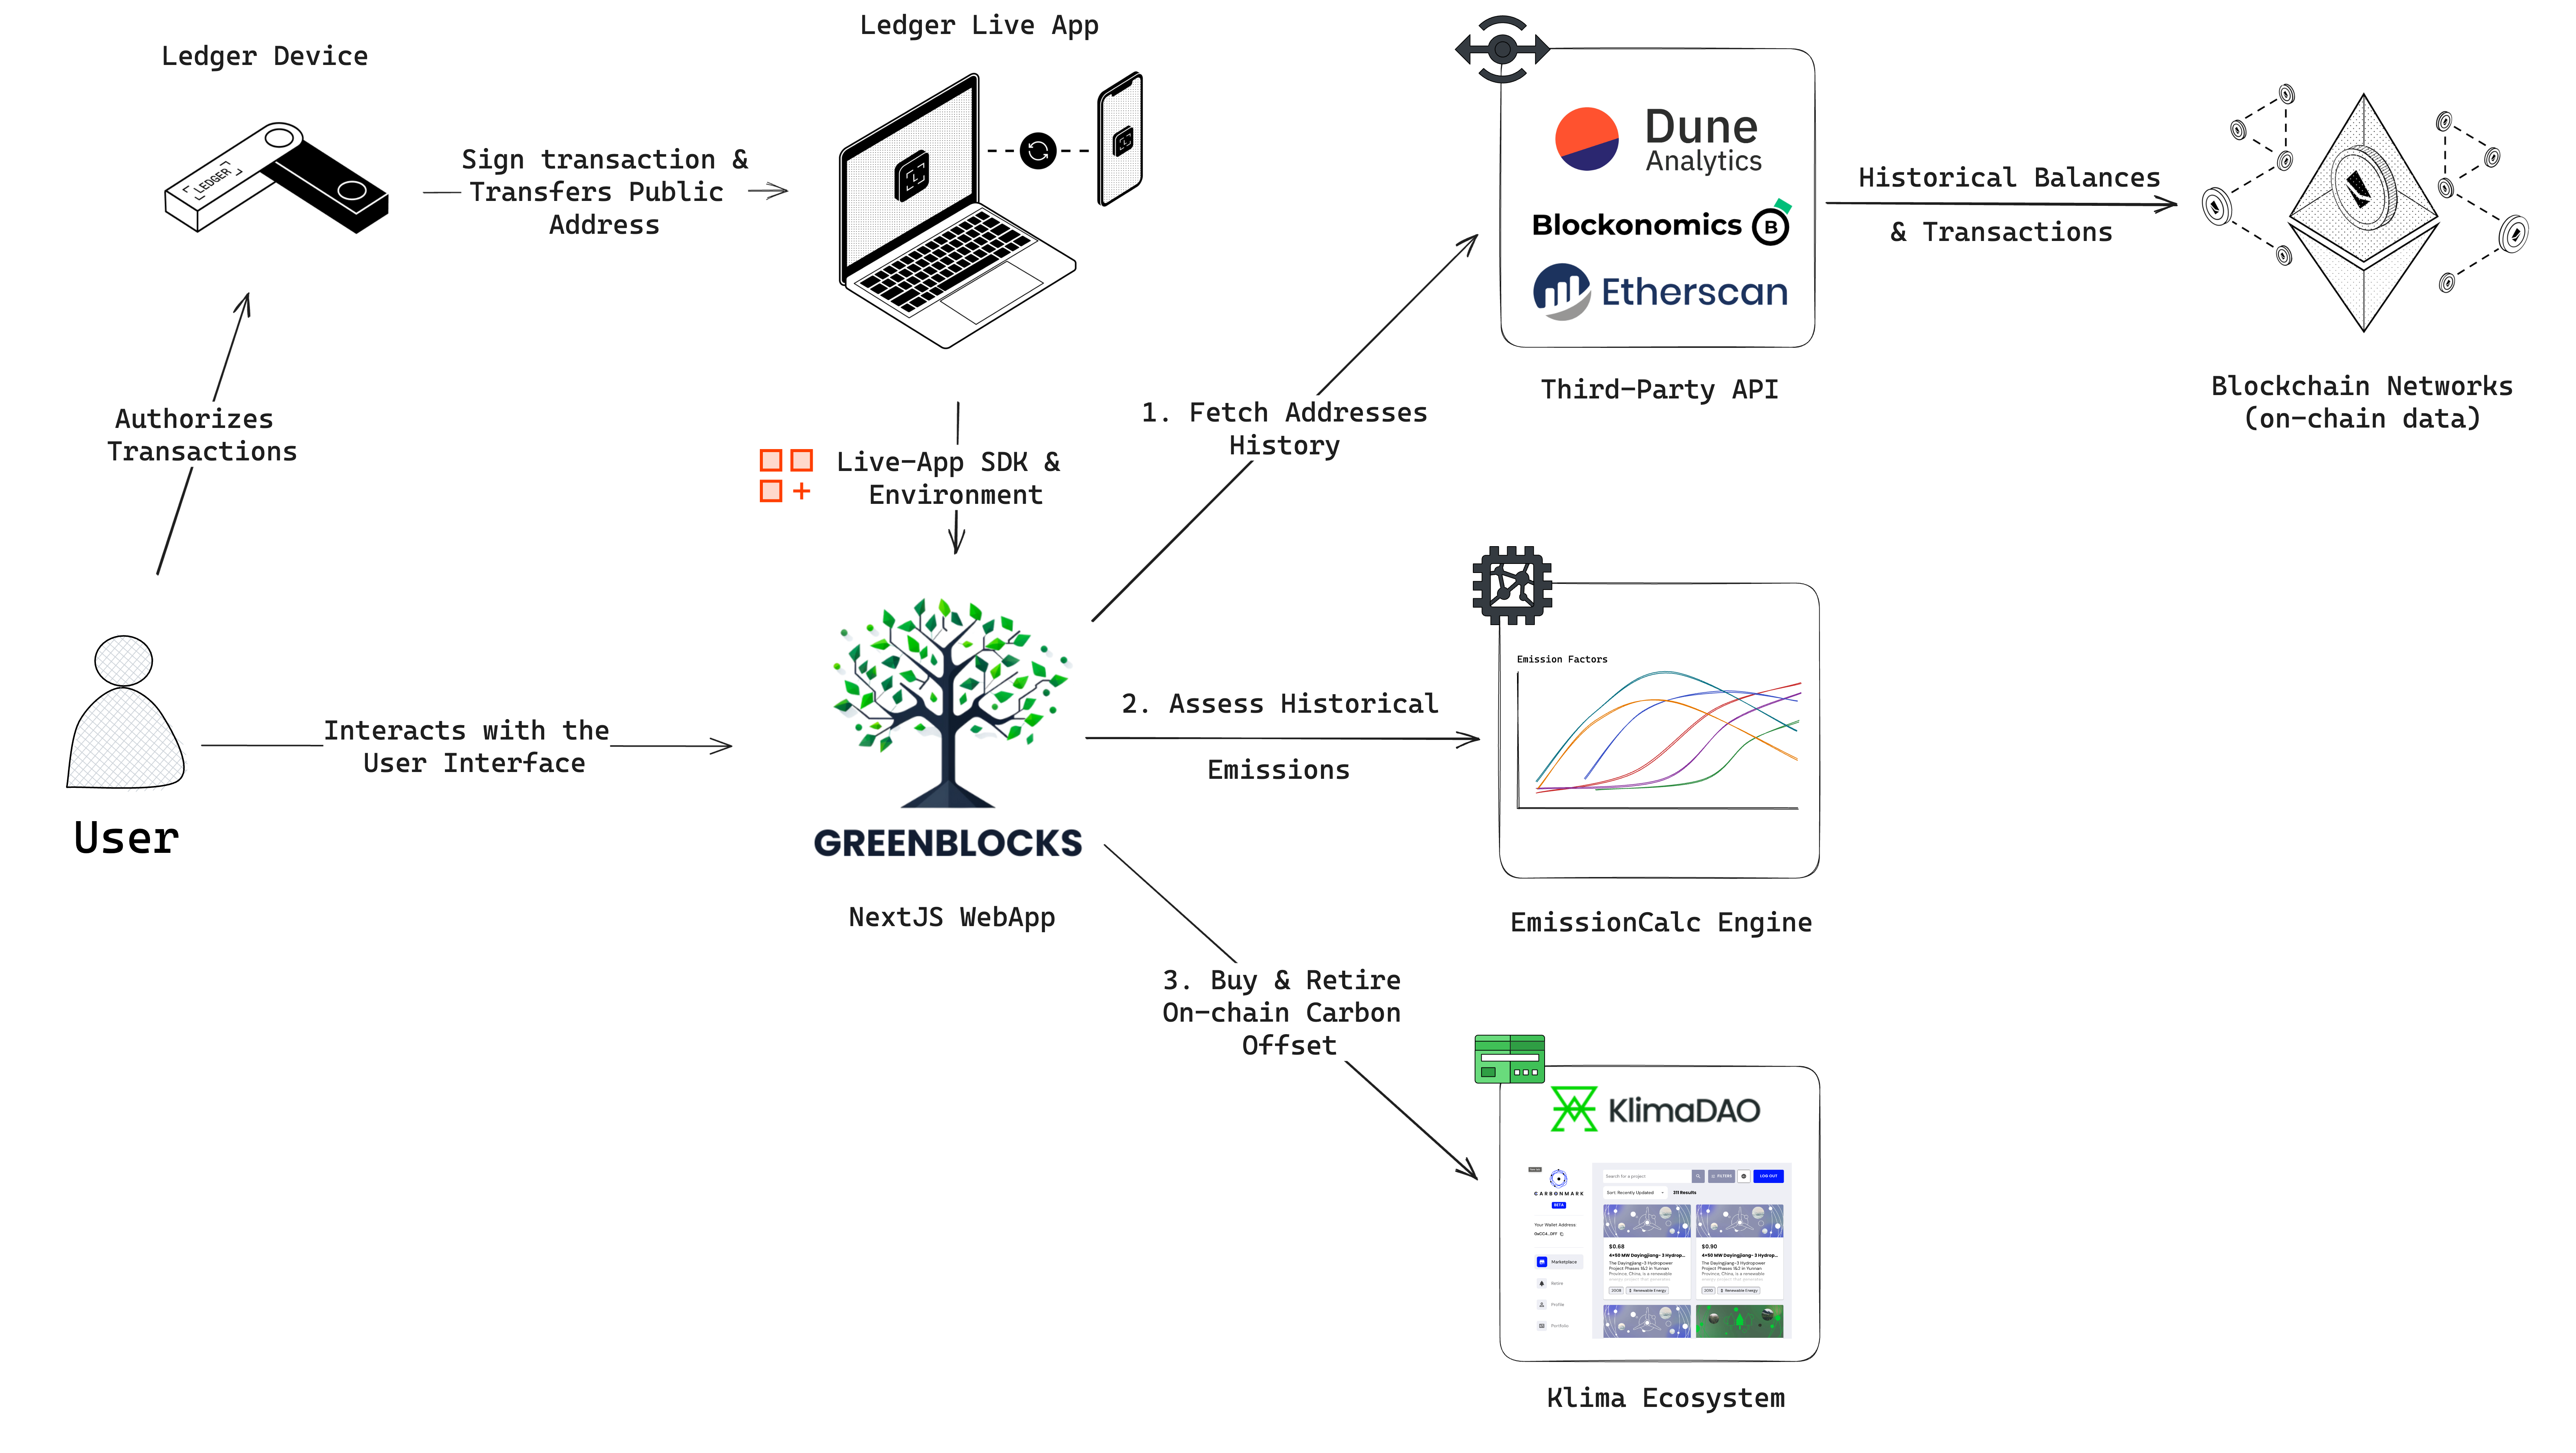
\includegraphics[scale=0.08]{figures/functionnal architecture.png}}
    \caption{GreenBlocks - Functionnal Architecture}
    \label{fig:functionnal_architecture}
\end{figure}

\begin{figure}[hbt!]
    \centering
    \centerline{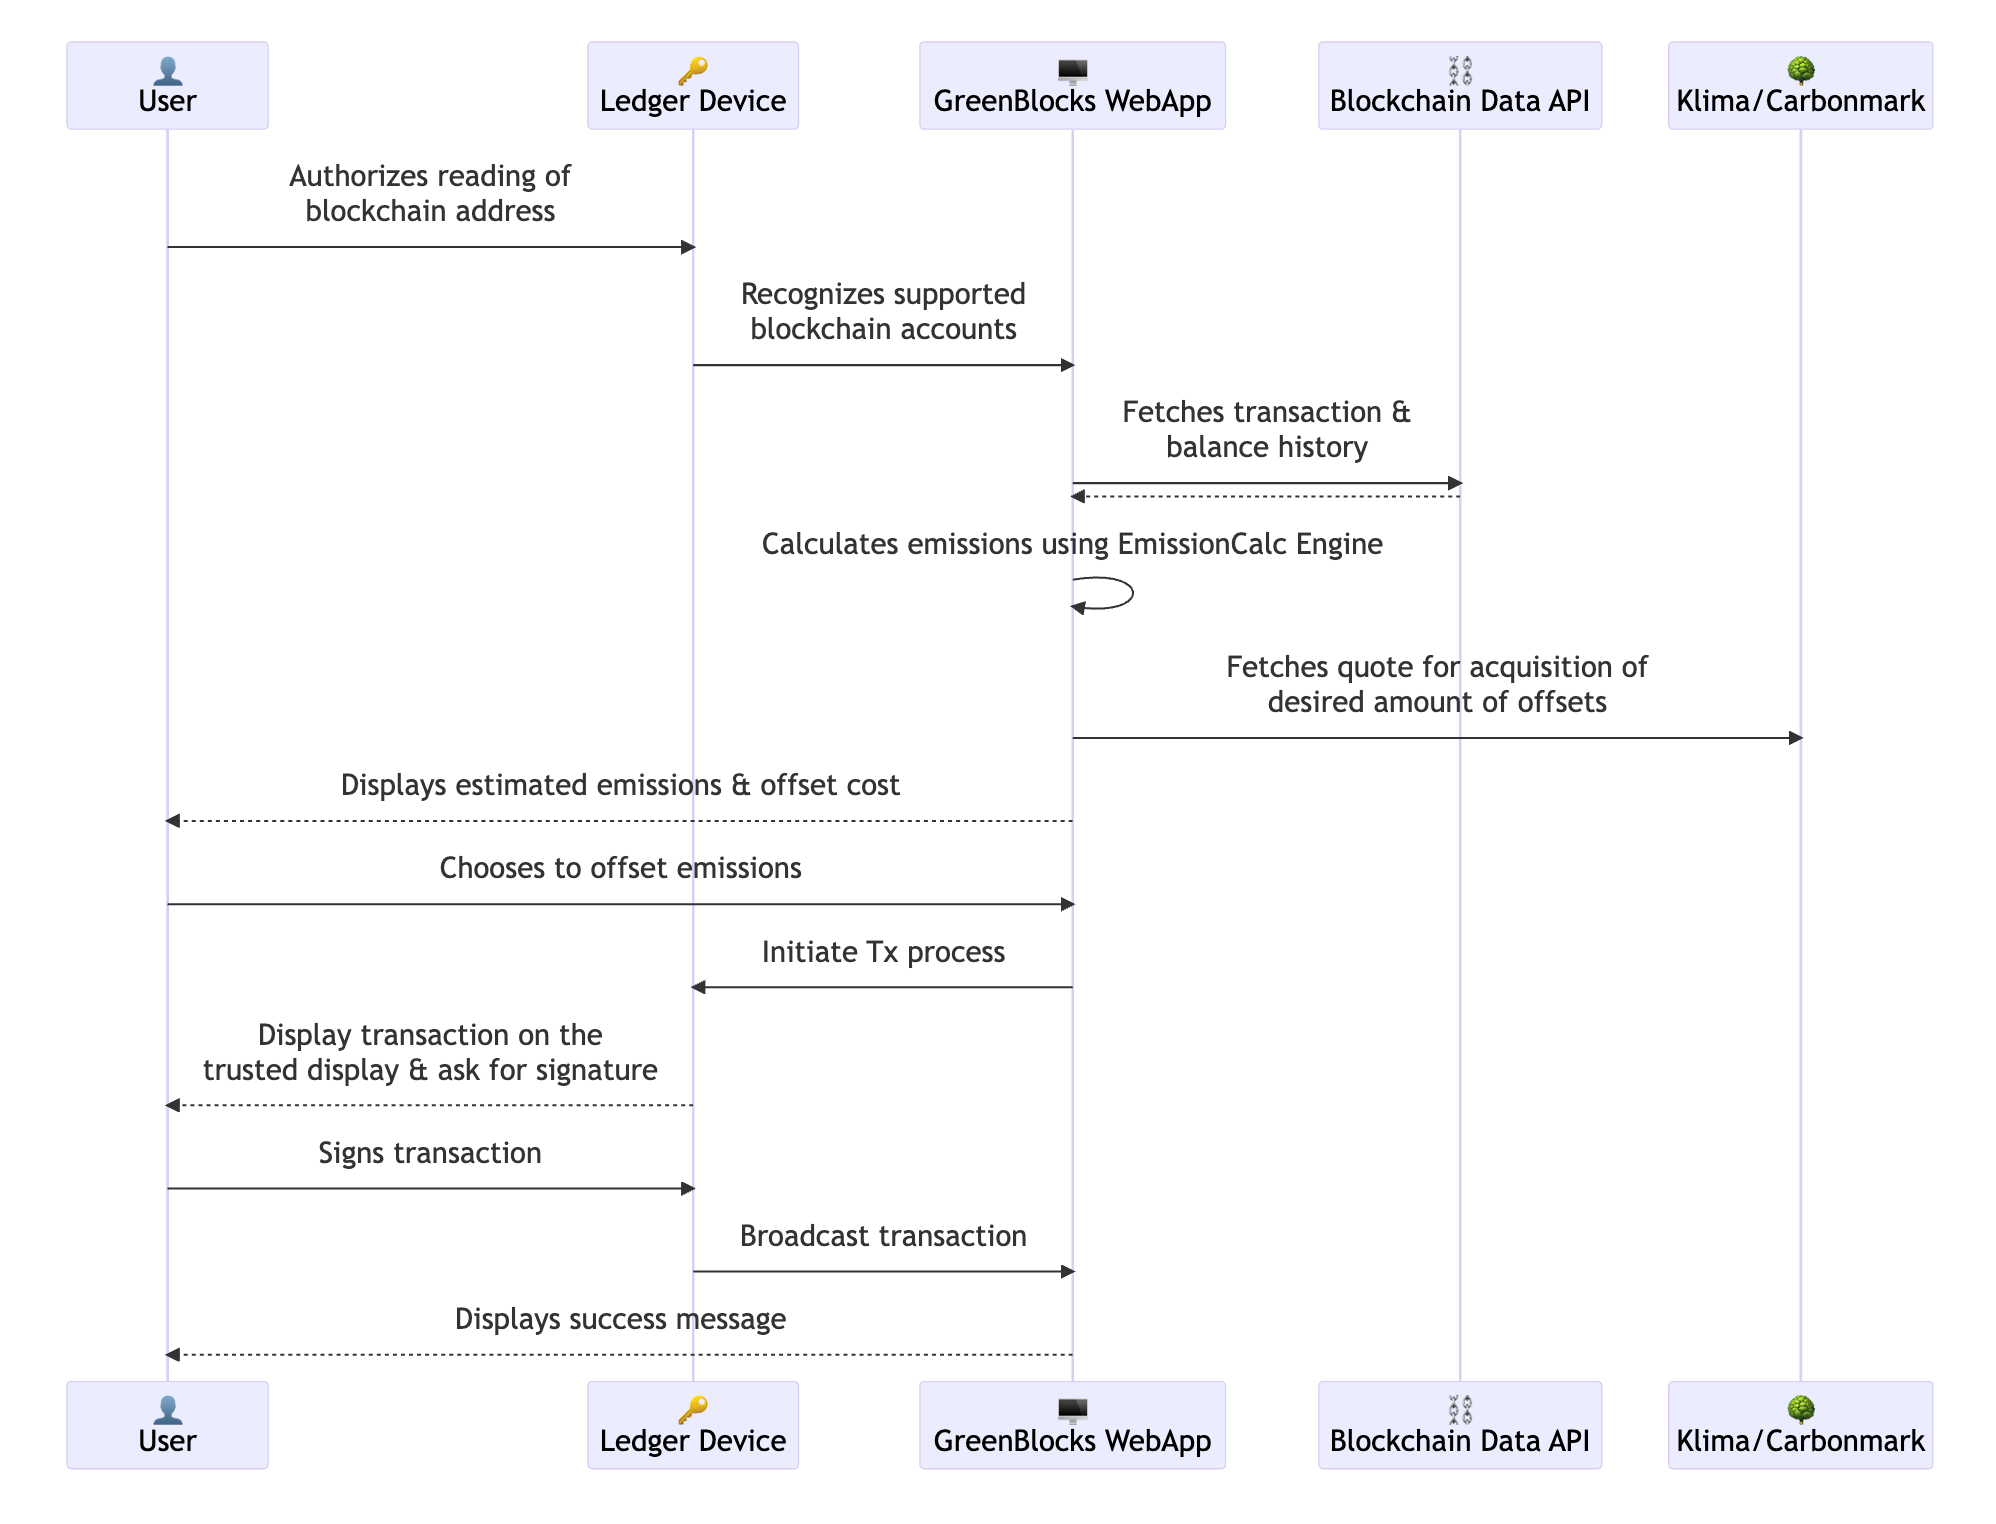
\includegraphics[scale=.27]{figures/sequence.png}}
    \caption{GreenBlocks - Sequence Diagram}
    \label{fig:sequence}
\end{figure}

\change{Review figure size for readability. Consider redo on lucid to control font}


\section{System Architecture and Components}
\subsection{User Interface Layer}
\subsection{Middleware Layer}
\subsection{Backend Layer}
\subsection{Data Layer}
\section{Development Process}

\chapter{Discussion}
\section{Results and Analysis}
\subsection{Validation and Sensitivity Analysis Results}
\subsubsection{Validation Results}
\subsubsection{Sensitivity Analysis Findings}
\section{Comparative Analysis: Different User Profiles and Protocols}
\section{Limitations and Future Work}
\section{Further Opportunities for Blockchain and Sustainability}

\chapter{Conclusion}


\bibliography{bibliography.bib}


\end{document}